\documentclass[12pt]{article}

\usepackage{sbc-template}
\usepackage{graphicx,url}
\usepackage[utf8]{inputenc}
\usepackage[brazil]{babel}
\usepackage{booktabs}
\usepackage{adjustbox}

\sloppy

\title{Replicação de Estratégias de Posicionamento de \textit{Registries}\\ para Redução do Tempo de Provisionamento de \textit{Containers}\\ na Computação de Borda}

\author{Felipe Torres, Gerson Gomes, Pedro Augusto Wagner\inst{1}}

\address{Escola Politécnica -- Pontifícia Universidade Católica do Rio Grande do Sul (PUCRS)\\
  Porto Alegre -- RS -- Brasil
  \email{\{felipe.torres, gerson.gomes, pedro.wagner\}@edu.pucrs.br}
}

\begin{document}

\maketitle

\begin{abstract}
  We reproduce, in the open-source EdgeSimPy simulator, the community-based
  registry placement strategy of Knob et al. (2021), which splits the network
  into bandwidth-balanced communities with the Fluid Communities algorithm and
  places one registry at the most central node of each community. We compare it
  against random placement on the two topologies of the original work (GARR and
  Erdős-Rényi) and extend the evaluation with a hexagonal cellular topology, the
  50 most downloaded Docker Hub images with their real layers, and a workload
  with Poisson arrivals, deadlines and an LRU layer cache. Across 1,360
  simulations, the community-based strategy provisioned containers faster than
  random placement in all 28 combinations of topology, image set and number of
  registries, with gains of up to 66\%, consistent with the up to 70\% reported
  in the original work. Under the original workload it never missed a deadline,
  whereas random placement occasionally led to catastrophic losses.
\end{abstract}

\begin{resumo}
  Reproduzimos, no simulador de código aberto EdgeSimPy, a estratégia de
  posicionamento de \textit{registries} baseada em comunidades de Knob et al.
  (2021), que divide a rede em comunidades balanceadas por banda com o algoritmo
  de comunidades fluidas e coloca um \textit{registry} no nó mais central de cada
  comunidade. Comparamos a estratégia com o posicionamento aleatório nas duas
  topologias do trabalho original (GARR e Erdős-Rényi) e estendemos a avaliação
  com uma topologia celular hexagonal, as 50 imagens mais baixadas do Docker Hub
  com suas camadas reais e uma carga de trabalho com chegadas de Poisson,
  \textit{deadline} e \textit{cache} LRU de camadas. Em 1.360 simulações, a
  estratégia baseada em comunidades provisionou os \textit{containers} mais
  rápido que o posicionamento aleatório nas 28 combinações de topologia,
  conjunto de imagens e número de \textit{registries}, com ganhos de até 66\%,
  coerentes com os até 70\% relatados no trabalho original. Sob a carga original,
  ela não perdeu nenhum \textit{deadline}, enquanto o posicionamento aleatório
  ocasionalmente levou a perdas catastróficas.
\end{resumo}

\section{Introdução}

A computação de borda (\textit{Edge Computing}) é uma tecnologia importante para
as redes 5G, pois aproxima o processamento do usuário final e viabiliza
aplicações sensíveis à latência, como realidade aumentada. Diferente da nuvem,
sua infraestrutura é distribuída, heterogênea e com recursos limitados. Cada vez
mais essas aplicações são executadas em \textit{containers}, cujas imagens têm
centenas de \textit{megabytes} e podem levar vários segundos para serem baixadas
em um nó de borda, de modo que o tempo de \textit{download} acaba dominando o
tempo total de instanciação.

Como a imagem é baixada de um \textit{registry} até o nó que vai executá-la, a
distância entre eles na topologia influencia esse tempo: quanto mais saltos e
enlaces congestionados o dado atravessa, maior o atraso. Por isso,
\textit{registries} bem posicionados podem reduzir o tempo de provisionamento sem
alterar a infraestrutura ou o orquestrador de \textit{containers}. O trabalho de
\cite{knob2021} propõe um posicionamento de \textit{registries} baseado em
comunidades e o avalia em um simulador próprio, cujo código não foi
disponibilizado.

Neste trabalho, reproduzimos essa estratégia no EdgeSimPy \cite{souza2023}, um
simulador de código aberto que modela o ciclo de vida de \textit{containers}, e
verificamos se os resultados se mantêm em uma ferramenta independente. Nossas
contribuições são: (i) uma implementação aberta do posicionamento baseado em
comunidades e do cenário experimental no EdgeSimPy \cite{repositorio}; (ii) a
reprodução dos experimentos nas topologias GARR e Erdős-Rényi; (iii) três
extensões que aproximam o cenário da prática: uma topologia celular hexagonal,
imagens reais do Docker Hub com camadas compartilhadas e uma carga de trabalho
com chegadas contínuas, \textit{deadline} e \textit{cache}; e (iv) o registro de
armadilhas do simulador que afetam qualquer experimento com imagens reais.

O restante do artigo está organizado assim: a Seção~\ref{sec:base} apresenta o
artigo base; a Seção~\ref{sec:metodologia}, os objetivos e a metodologia; a
Seção~\ref{sec:implementacao}, a implementação; a Seção~\ref{sec:config}, a
configuração experimental; a Seção~\ref{sec:resultados}, os resultados; a
Seção~\ref{sec:discussao}, a discussão e as ameaças à validade; e as
Seções~\ref{sec:impacto} e~\ref{sec:conclusao}, o impacto e as conclusões.

\section{Artigo Base e Trabalhos Relacionados}
\label{sec:base}

O trabalho que serve de base é ``Community-based Placement of Registries to Speed
up Application Deployment on Edge Computing'', de Luis A. D. Knob, Francescomaria
Faticanti, Tiago Ferreto e Domenico Siracusa, publicado em 2021 na
\textit{IEEE International Conference on Cloud Engineering} (IC2E), p. 147--153,
DOI 10.1109/IC2E52221.2021.00029, disponível em
\url{https://ieeexplore.ieee.org/document/9610275} (XX citações segundo o Google
Scholar) \cite{knob2021}.

O artigo trata da redução da latência de \textit{deployment} na borda a partir do
posicionamento dos \textit{registries}, que armazenam as imagens dos
\textit{containers}. O problema é NP-difícil, por ser um particionamento de
grafos, e os autores propõem uma heurística de duas fases: o algoritmo de
comunidades fluidas (FluidC) \cite{pares2017} com busca \textit{Hill-Climbing}
divide a rede em comunidades balanceadas por banda; em cada comunidade, o nó de
maior centralidade de autovetor hospeda um \textit{registry}. Validada por
simulação nas topologias Erdős-Rényi (aleatória) e GARR (rede real italiana), a
solução reduziu o tempo de instanciação em até 70\% no melhor caso. Outros
trabalhos, como \cite{darrous2019}, também tratam do posicionamento de imagens na
borda, mas costumam depender de nós potentes e redes rápidas, nem sempre
realistas em cenários geodistribuídos. O EdgeSimPy \cite{souza2023}, que
utilizamos, é um \textit{framework} em Python que modela o ciclo de vida
completo de \textit{containers} (imagens, camadas e \textit{registries}), o que o
torna adequado ao nosso problema.

\section{Objetivos e Metodologia}
\label{sec:metodologia}

O objetivo geral é reproduzir e avaliar, no EdgeSimPy, a estratégia de
posicionamento baseado em comunidades de \cite{knob2021}. A pergunta de pesquisa
principal é: \textbf{os resultados obtidos ao reproduzir essa estratégia no
EdgeSimPy são consistentes com os relatados por \cite{knob2021}, em termos de
tempo de provisionamento e de \textit{containers} não iniciados?} Como pergunta
secundária, investigamos se a vantagem da estratégia se mantém em condições mais
próximas da prática: outra classe de topologia, imagens reais e chegadas
contínuas de requisições.

O trabalho seguiu as etapas: (1) configurar os cenários (topologias e parâmetros
de simulação); (2) implementar no EdgeSimPy a estratégia baseada em comunidades
e a estratégia aleatória usada como comparação; (3) executar as simulações
variando a quantidade de \textit{registries} ($K$); (4) coletar o tempo de
provisionamento e a fração de \textit{containers} não iniciados no prazo; e (5)
comparar os resultados com os do trabalho original. Todas as comparações são
pareadas: em uma mesma \textit{seed}, as duas estratégias recebem o mesmo grafo,
os mesmos serviços e as mesmas imagens, e só muda a posição dos
\textit{registries}.

\section{Implementação}
\label{sec:implementacao}

A implementação usa o EdgeSimPy \cite{souza2023} e a biblioteca NetworkX, ambos
de código aberto (\url{https://github.com/EdgeSimPy/EdgeSimPy} e
\url{https://networkx.org}), e está disponível no repositório do grupo
\cite{repositorio}. O compartilhamento de banda entre fluxos concorrentes usa o
algoritmo \textit{max-min fairness} já disponível no EdgeSimPy.

\textbf{Posicionamento baseado em comunidades.} A primeira fase executa o FluidC
repetidas vezes, com sementes diferentes, e mantém a partição em $K$ comunidades
com o menor desvio-padrão da banda interna (soma da banda dos enlaces com as duas
extremidades na mesma comunidade), descartando partições com alguma comunidade
sem enlace interno. A busca para após 100 execuções consecutivas sem melhora. O
pseudocódigo original não atualiza o melhor desvio ao aceitar uma partição
melhor; seguimos a descrição textual (``até não haver comunidades melhores'') e
fazemos a atualização. A segunda fase escolhe, em cada comunidade, o nó de maior
centralidade de autovetor no subgrafo da comunidade. O \textbf{posicionamento
aleatório} sorteia $K$ nós distintos.

\textbf{Cenários.} Cada nó da topologia recebe uma estação-base e um servidor de
borda. Cada \textit{registry} fica em um servidor dedicado, ligado ao nó escolhido
por um enlace de 10~Gbps e sem capacidade para executar serviços. Todos os
\textit{registries} guardam todas as imagens, e cada servidor baixa cada camada do
\textit{registry} mais próximo em número de saltos.

\textbf{Resolução temporal.} O EdgeSimPy desconta de cada fluxo, a cada passo de
simulação (\textit{tick}), um volume igual à banda alocada, sem considerar a
duração do passo. Por isso, gravamos a banda no cenário em MB por \textit{tick}
(banda em MB/s multiplicada pela duração do \textit{tick}) e usamos
\textit{ticks} de 0,1~s em todos os experimentos. Com as imagens do artigo
(200~MB em uma camada), \textit{ticks} de 1~s alteram o tempo medido em cerca de
2\%; com imagens reais, em que a maioria das camadas é pequena, quase todo
\textit{download} termina dentro do primeiro \textit{tick} de 1~s e o tempo medido
se reduz ao custo fixo do simulador, tornando as estratégias indistinguíveis.

\textbf{Armadilhas do simulador.} Além da resolução temporal, encontramos um
comportamento que afeta imagens reais: se uma imagem lista a mesma camada duas
vezes (como a camada vazia padrão do Docker), o EdgeSimPy coloca duas cópias dela
na fila do servidor, e outra imagem que use a mesma camada no mesmo servidor
nunca termina de ser provisionada, porque o simulador compara a contagem de
camadas baixadas com o tamanho da lista. Nosso gerador remove as repetições. Em
simulações longas, também retiramos das listas internas do simulador os fluxos
concluídos e as camadas removidas do \textit{cache}, que de outro modo tornam
cada passo progressivamente mais lento.

\section{Configuração Experimental}
\label{sec:config}

A Tabela~\ref{tab:topologias} resume as topologias. A \textbf{GARR do artigo} é
a versão usada por \cite{knob2021}, fornecida pelo professor da disciplina, com
banda própria em cada enlace; o arquivo tem 112 enlaces, um deles duplicado, que
descartamos. A \textbf{GARR do Topology Zoo} \cite{knight2011} (mapa de 2011) foi
a versão pública que usamos antes de obter a do artigo e fica como comparação.
A \textbf{Erdős-Rényi} $G(n,p)$ usa $n = 100$ e $p = 0{,}049$, o que dá em média
242 enlaces; cada \textit{seed} gera um grafo diferente, sorteado novamente se
sair desconexo. A \textbf{hexagonal} é uma malha de células no estilo de rede
celular, em que cada célula se liga às até seis vizinhas, seguindo a mesma
convenção do gerador de cenários do EdgeSimPy; ela tem o tamanho da Erdős-Rényi,
mas diâmetro mais que duas vezes maior.

\begin{table}[ht]
\centering
\caption{Topologias avaliadas.}
\label{tab:topologias}
\small
\begin{adjustbox}{max width=\textwidth}
\begin{tabular}{lrrrrl}
\toprule
Topologia & Nós & Enlaces & Grau médio & Diâmetro & Banda dos enlaces \\
\midrule
GARR do artigo & 70 & 111 & 3,17 & 9 & do arquivo (1 a 100~Gbps) \\
GARR do Topology Zoo & 61 & 75 & 2,46 & 8 & 1~Gbps \\
Erdős-Rényi $G(100;\,0{,}049)$ & 100 & $\approx$244 & $\approx$4,9 & 5 a 7 & 1~Gbps \\
Hexagonal $10\times10$ & 100 & 261 & 5,22 & 14 & 1~Gbps \\
\bottomrule
\end{tabular}
\end{adjustbox}
\end{table}

Usamos dois conjuntos de imagens. As \textbf{imagens fictícias do artigo} são 13
imagens de 200~MB com uma camada cada. As \textbf{imagens reais} são as 50 mais
baixadas do Docker Hub \cite{dockerhub}, com o tamanho comprimido de cada camada
(o que trafega em um \textit{download}): vão de 0,002~MB a 503~MB e somam 290
camadas distintas e 5,0~GB. Camadas com o mesmo identificador são compartilhadas:
o servidor não baixa novamente uma camada que já possui.

Cada servidor de borda tem 32 núcleos e 32~GB de memória, executa até quatro
\textit{containers} (8 núcleos e 8~GB cada) e baixa até três camadas
simultaneamente. Avaliamos $K \in \{1, 2, 4, 8\}$ em dois modos:

\begin{itemize}
  \item \textbf{Rajada:} 60 serviços pedem provisionamento ao mesmo tempo, cada um
  com imagem e estação-base sorteadas de modo uniforme, e um escalonador aleatório
  escolhe o servidor entre os que têm capacidade. A métrica é o tempo médio de
  provisionamento dos 60 serviços. Usamos 20 \textit{seeds} por combinação.
  \item \textbf{Carga de trabalho do artigo:} requisições chegam por um processo
  de Poisson com 5 requisições/s (o valor do artigo), 10 e 20 requisições/s, com
  \textit{deadline} de 25~s, \textit{cache} LRU de 600~MB por servidor e as
  imagens do Docker Hub, na GARR do artigo. A métrica é a fração de requisições
  cujo \textit{container} não estava em execução até o \textit{deadline}. O artigo
  não informa por quanto tempo cada \textit{container} executa; adotamos 30~s,
  pois sem liberar espaço os servidores lotam em poucos minutos. Cada simulação
  tem 10 minutos de chegadas, e usamos 10 \textit{seeds} por combinação.
\end{itemize}

Para cada par (FluidC, aleatório) de uma mesma \textit{seed}, calculamos o ganho
$1 - t_{\mathrm{FluidC}}/t_{\mathrm{aleatório}}$ e contamos as vitórias, empates
e derrotas do FluidC (V/E/D). A significância é avaliada com um teste de
permutação pareado exato (troca de sinais das diferenças, bicaudal).

\section{Resultados}
\label{sec:resultados}

No total, executamos 1.360 simulações: 1.120 no modo rajada (4 topologias com
imagens fictícias e 3 com imagens reais, 4 valores de $K$, 2 estratégias e 20
\textit{seeds}) e 240 com a carga de trabalho do artigo. Nenhuma simulação falhou.

\subsection{Modo rajada com as imagens do artigo}

A Figura~\ref{fig:tempo} mostra o tempo médio de provisionamento e a
Tabela~\ref{tab:rajada} resume a comparação. O FluidC foi mais rápido, em média,
em todas as topologias e valores de $K$, com diferença significativa em todas as
combinações ($p < 0{,}05$; na maioria, $p < 0{,}001$).

\begin{figure}[ht]
\centering
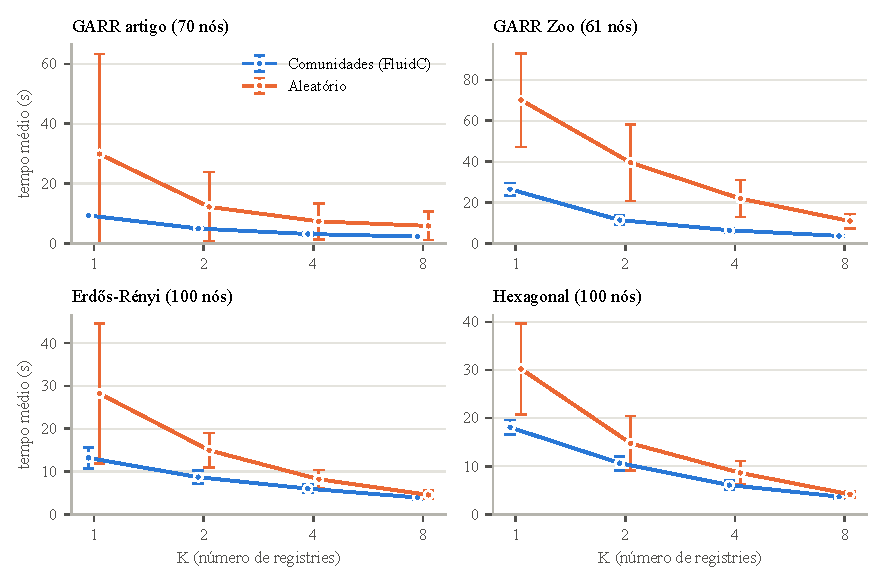
\includegraphics[width=\textwidth]{figuras/tempo_por_k.pdf}
\caption{Tempo médio de provisionamento no modo rajada com as imagens do artigo
(média $\pm$ desvio-padrão de 20 \textit{seeds}).}
\label{fig:tempo}
\end{figure}

\begin{table}[ht]
\centering
\caption{Modo rajada: tempo médio de provisionamento em segundos (FluidC /
aleatório) e, entre parênteses, o ganho médio do FluidC em 20 \textit{seeds}.
$^\dagger$Distribuição bimodal: FluidC venceu/empatou/perdeu em 6/14/0
(imagens do artigo) e 7/13/0 (Docker Hub) \textit{seeds}.}
\label{tab:rajada}
\small
\begin{adjustbox}{max width=\textwidth}
\begin{tabular}{lllll}
\toprule
Topologia & $K=1$ & $K=2$ & $K=4$ & $K=8$ \\
\midrule
\multicolumn{5}{l}{\textit{Imagens do artigo (13 $\times$ 200~MB)}} \\
GARR do artigo & 9,3 / 29,9 (26\%)$^\dagger$ & 5,0 / 12,2 (39\%) & 3,1 / 7,4 (43\%) & 2,3 / 5,8 (43\%) \\
GARR Zoo & 26,5 / 70,1 (54\%) & 11,4 / 39,5 (65\%) & 6,4 / 21,9 (66\%) & 3,7 / 10,9 (63\%) \\
Erdős-Rényi & 13,2 / 28,2 (44\%) & 8,7 / 14,9 (38\%) & 6,0 / 8,2 (24\%) & 3,9 / 4,5 (10\%) \\
Hexagonal & 18,1 / 30,2 (35\%) & 10,6 / 14,8 (22\%) & 6,1 / 8,6 (25\%) & 3,7 / 4,1 (9\%) \\
\midrule
\multicolumn{5}{l}{\textit{Top 50 imagens do Docker Hub}} \\
GARR do artigo & 3,1 / 10,1 (26\%)$^\dagger$ & 1,8 / 4,2 (36\%) & 1,3 / 2,4 (38\%) & 1,0 / 2,0 (35\%) \\
Erdős-Rényi & 4,8 / 9,7 (40\%) & 3,4 / 5,3 (32\%) & 2,5 / 3,0 (17\%) & 1,8 / 1,9 (6\%) \\
Hexagonal & 6,5 / 10,6 (34\%) & 4,1 / 5,5 (20\%) & 2,5 / 3,4 (22\%) & 1,7 / 1,9 (7\%) \\
\bottomrule
\end{tabular}
\end{adjustbox}
\end{table}

Nas duas versões da GARR o ganho fica alto para qualquer $K$ (de 39\% a 66\%,
exceto $K = 1$ na GARR do artigo). Uma rede acadêmica tem núcleo e periferia, e um
\textit{registry} sorteado na periferia concentra o tráfego nos poucos caminhos
disponíveis. Na Erdős-Rényi e na hexagonal o ganho cai com $K$, de 35--44\% em
$K = 1$ para 9--10\% em $K = 8$: com oito \textit{registries} em cem nós, mesmo
um sorteio deixa quase todos os nós perto de algum \textit{registry}. O FluidC
também é mais previsível: na maior parte das combinações, o desvio-padrão do
posicionamento aleatório entre \textit{seeds} passa de duas vezes o do FluidC.

A Figura~\ref{fig:ganho} mostra o ganho em cada \textit{seed}. O caso $K = 1$ na
GARR do artigo merece atenção: com um único \textit{registry}, o FluidC se reduz à
escolha do nó de maior centralidade. Em 14 das 20 \textit{seeds} o sorteio cai em
um nó do núcleo de 10~Gbps e empata exatamente com o FluidC; nas outras 6, cai em
um nó mal conectado e perde por 79\% a 89\%. A média de 26\% descreve mal essa
distribuição bimodal, por isso reportamos também V/E/D.

\begin{figure}[ht]
\centering
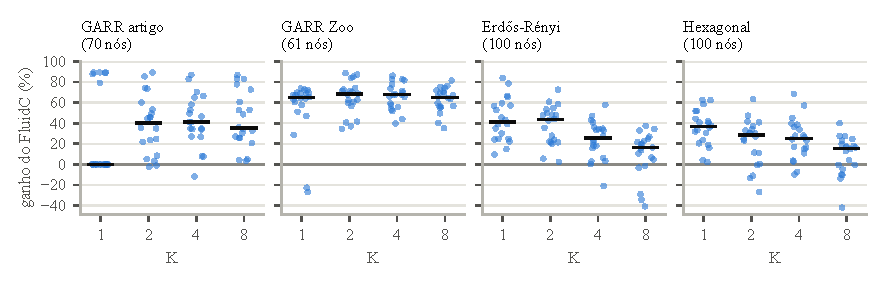
\includegraphics[width=\textwidth]{figuras/ganho_por_seed.pdf}
\caption{Ganho do FluidC sobre o aleatório em cada \textit{seed} (imagens do
artigo); o traço indica a mediana.}
\label{fig:ganho}
\end{figure}

\subsection{Modo rajada com imagens reais}

Com as imagens do Docker Hub (parte inferior da Tabela~\ref{tab:rajada}), os
tempos caem para 33--47\% dos obtidos com as imagens do artigo, porque as imagens
reais são, em média, menores e as camadas compartilhadas não são baixadas
novamente. O ganho relativo do FluidC, porém, muda pouco: continua alto na GARR
(26--38\%) e decrescente com $K$ na Erdős-Rényi e na hexagonal. Todas as 12
combinações têm diferença significativa ($p < 0{,}05$).

\subsection{Carga de trabalho do artigo}

A Figura~\ref{fig:carga} e a Tabela~\ref{tab:carga} mostram a fração de
requisições não iniciadas no prazo. Com 5 requisições/s, a taxa do artigo, o
FluidC não perdeu nenhuma requisição em nenhuma \textit{seed}, com tempo médio até
o \textit{container} executar de 0,5 a 0,6~s. O posicionamento aleatório também
não perdeu requisições na maioria das \textit{seeds}, mas em 2 ou 3 de cada 10 o
\textit{registry} ficou atrás de um enlace fraco e as perdas chegaram a 18\% com
$K \geq 2$ e a 87--95\% com $K = 1$. Como só essas poucas \textit{seeds} diferem,
a diferença ainda não é estatisticamente significativa ($p = 0{,}25$).

\begin{figure}[ht]
\centering
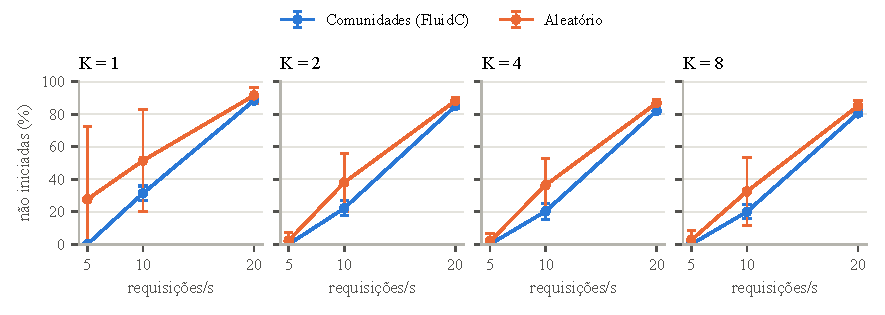
\includegraphics[width=\textwidth]{figuras/carga.pdf}
\caption{Requisições não iniciadas no prazo em função da taxa de chegada (GARR do
artigo, imagens do Docker Hub; média $\pm$ desvio-padrão de 10 \textit{seeds}).}
\label{fig:carga}
\end{figure}

\begin{table}[ht]
\centering
\caption{Carga de trabalho: requisições não iniciadas no prazo (\%, FluidC /
aleatório) e $p$-valor do teste pareado (10 \textit{seeds}).}
\label{tab:carga}
\small
\begin{adjustbox}{max width=\textwidth}
\begin{tabular}{lccc}
\toprule
$K$ & 5 req./s & 10 req./s & 20 req./s \\
\midrule
1 & 0,0 / 27,7 ($p = 0{,}25$) & 31,3 / 51,5 ($p = 0{,}08$) & 88,5 / 91,6 ($p = 0{,}018$) \\
2 & 0,0 / 2,2 ($p = 0{,}25$) & 22,1 / 38,0 ($p = 0{,}006$) & 85,0 / 88,3 ($p = 0{,}002$) \\
4 & 0,0 / 1,9 ($p = 0{,}25$) & 20,3 / 36,4 ($p = 0{,}002$) & 82,1 / 87,0 ($p = 0{,}004$) \\
8 & 0,0 / 2,6 ($p = 0{,}50$) & 20,0 / 32,5 ($p = 0{,}018$) & 80,6 / 85,1 ($p = 0{,}004$) \\
\bottomrule
\end{tabular}
\end{adjustbox}
\end{table}

Com 10 requisições/s, acima da capacidade de processamento da infraestrutura
(cerca de 9 requisições/s com \textit{containers} de 30~s), as duas estratégias
perdem requisições, mas o FluidC perde de 12 a 16 pontos percentuais a menos com
$K \geq 2$ (diferença significativa). Com 20 requisições/s o processamento satura
e ambas perdem mais de 80\%, ainda com vantagem de 3 a 5 pontos para o FluidC. A
taxa de acerto do \textit{cache} de 600~MB ficou entre 11\% e 15\% nas duas
estratégias: com 50 imagens sorteadas de modo uniforme, cada servidor guarda
poucas imagens.

\section{Discussão e Ameaças à Validade}
\label{sec:discussao}

\textbf{Consistência com o trabalho original.} Respondendo à pergunta de pesquisa,
os resultados são qualitativamente consistentes com \cite{knob2021}: o
posicionamento baseado em comunidades reduziu o tempo de provisionamento em todas
as configurações, com ganho máximo de 66\% (GARR do Topology Zoo, $K = 4$),
próximo dos até 70\% relatados. A extensão mostra que a vantagem se mantém com
imagens reais e em uma topologia celular, e que, sob a carga do artigo, ela
aparece menos na média e mais na eliminação do risco de configurações
catastróficas.

As principais ameaças à validade são:
\begin{itemize}
  \item \textbf{Escalonador.} Usamos um escalonador aleatório; o artigo também
  avalia o escalonador PESS, que ainda não implementamos.
  \item \textbf{Parâmetros não informados.} O tempo de execução dos
  \textit{containers} (30~s), o \textit{deadline} fixo de 25~s e a capacidade dos
  servidores (quatro \textit{containers}) são suposições nossas, que afetam
  diretamente a fração de requisições não iniciadas a 10 e 20 requisições/s.
  \item \textbf{Duração e repetições da carga.} As simulações da carga têm 10
  minutos, e não uma hora como no artigo, e com 10 \textit{seeds} a diferença a
  5 requisições/s não é significativa.
  \item \textbf{Topologias.} A GARR do artigo tem 111 enlaces, e não 112, após
  descartar um enlace duplicado. Na Erdős-Rényi, sortear novamente os grafos
  desconexos favorece grafos com um pouco mais de enlaces.
  \item \textbf{Imagens.} A coleta do Docker Hub usa a \textit{tag}
  \texttt{latest} quando disponível e, nos demais casos, a versão mais recente, o
  que incluiu algumas versões de desenvolvimento; uma das imagens veio com tamanho
  aparentemente incorreto (0,04~MB).
  \item \textbf{Simulador.} As armadilhas da Seção~\ref{sec:implementacao} mostram
  que detalhes do EdgeSimPy podem mascarar o efeito do posicionamento; os
  contornamos e documentamos, mas outros comportamentos podem existir.
\end{itemize}

\section{Impacto e Conexão com a Sociedade}
\label{sec:impacto}

Reduzir o tempo de provisionamento de \textit{containers} na borda é relevante
para aplicações que dependem de baixa latência. Um provisionamento mais rápido
beneficia áreas como as redes 5G, a Internet das Coisas, a realidade aumentada e
as cidades inteligentes, além de operadoras de telecomunicações e provedores de
serviços de borda, que precisam instanciar aplicações de forma ágil em
infraestruturas distribuídas e limitadas. Nossos resultados indicam que um bom
posicionamento de \textit{registries}, sem nenhuma mudança na infraestrutura,
reduz o tempo de provisionamento e, principalmente, evita configurações em que um
único \textit{registry} mal posicionado compromete o atendimento. A
implementação, os cenários e os resultados estão disponíveis publicamente
\cite{repositorio}, e todas as etapas foram registradas no caderno de pesquisa
digital.

\section{Conclusão e Trabalhos Futuros}
\label{sec:conclusao}

Reproduzimos no EdgeSimPy o posicionamento de \textit{registries} baseado em
comunidades de \cite{knob2021} e confirmamos sua vantagem sobre o posicionamento
aleatório em quatro topologias, com imagens fictícias e reais e sob uma carga de
trabalho com chegadas contínuas. Como trabalhos futuros, pretendemos: implementar
o escalonador PESS; executar a carga de trabalho com uma hora de simulação e mais
\textit{seeds}; validar os parâmetros não informados no artigo original; e, com
essa base, propor e avaliar uma nova estratégia de posicionamento.

\bibliographystyle{sbc}
\bibliography{sbc-template}

\end{document}
